
\documentclass{llncs}
\usepackage{times}
\usepackage[T1]{fontenc}
\usepackage{mdframed}
\usepackage{a4}
\usepackage[portuguese]{babel}
\usepackage[utf8]{inputenc}
\usepackage[T1]{fontenc}
\usepackage{epstopdf}
\usepackage{graphicx}
\usepackage{subfig}
\usepackage{fancyhdr}
\usepackage{amsmath}
\usepackage{float}
\usepackage{indentfirst}
\setcounter{tocdepth}{4}
\makeatletter
\setcounter{page}{1}
\renewcommand\subsubsection{\@startsection{subsubsection}{3}{\z@}%
                       {-18\p@ \@plus -4\p@ \@minus -4\p@}%
                       {0.5em \@plus 0.22em \@minus 0.1em}%
                       {\normalfont\normalsize\bfseries\boldmath}}
\makeatother
\usepackage{textcomp}
\definecolor{light-gray}{gray}{0.95}
\setcounter{secnumdepth}{3}%\renewcommand{\baselinestretch}{1.5}
\topmargin=-0.6in
\evensidemargin=0in
\oddsidemargin=0in
\textwidth=6.5in
\textheight=9.3in
\headsep=0.25in
% Set up the header and footer
\pagestyle{plain}


\begin{document}

\mainmatter
\title{Sistemas Distribuídos \newline Trabalho Prático}

\titlerunning{Relatório do Trabalho Prático}

\author{Daniel da Silva Fernandes - A78377 \and \newline Maria Helena Ribeiro Poleri - A78633 \and \newline Mariana Martins de Sá Miranda - A77782 \and \newline Pedro Henrique Moreira Gomes Fernandes - A77377}

\authorrunning{Daniel da Silva Fernandes - A77377 
	\and Maria Helena Ribeiro Poleri - A78633 
	\and Mariana Martins de Sá Miranda - A77782 
	\and Pedro Henrique Moreira Gomes Fernandes - A77377}

\institute{
Universidade do Minho, Departamento de Informática, 4710-057 Braga, Portugal\\
e-mail: \{a78377, a78633, 77782, 77377\}@alunos.uminho.pt
}

\date{3 de Janeiro de 2018}
\bibliographystyle{splncs}

\maketitle
\makeatletter
\let\ps@oldempty\ps@empty % save default definition of \ps@empty
\renewcommand\ps@empty\ps@plain
\makeatother
\begin{abstract}
Trabalho prático que consiste no desenvolvimento de uma aplicação distribuída para \textit{matchmaking} num jogo online por equipas, semelhante ao Overwatch. 
A funcionalidade essencial é composta por duas fases: 
1) formar as duas equipas para jogar cada partida; 
2) a fase em que cada jogador escolhe qual o herói com que joga, antes do jogo começar. 
Os utilizadores devem poder interagir, usando um cliente escrito em Java, intermediados por um servidor \textit{multi-threaded} também escrito em Java, e recorrendo a comunicação via sockets TCP.
\end{abstract}

\section{Introdução}

Neste relatório pretendemos descrever elementos e o processo de desenvolvimento
de uma aplicação distribuída que se serve da arquitetura Servidor-Cliente. Serão 
abordadas algumas das classes que constituem algumas das estruturas usadas para 
este projeto, assim como serão descritos eventos e procedimentos seguidos para que 
os primeiros ocorram com sucesso. Cada jogador na aplicação será tido como um cliente 
e para eles existirá um servidor, que terá como função gerir os seus pedidos e oferecer 
as funcionalidades que um sistema de \textit{matchmaking} e simulação de jogo envolvem.
 
A ligação entre clientes e servidor será efetuada recorrendo a \textit{sockets} TCP, 
disponibilizados pelas bibliotecas da linguagem de programação utilizada, Java, e 
vários procedimentos, entre os quais se encontram os de leitura e escrita, ficarão sob 
a responsabilidade de \textit{threads} criadas para esse fim. Pretendemos com este trabalho 
prático suportar todas as funcionalidades sugeridas no enunciado e garantir o 
sucesso do sistema aqui criado.

\section{Lógica do Servidor}

\subsection{Player.java}

Os elementos centrais deste projeto são os jogadores. Cada um deles terá um objeto dedicado, que 
corresponderá a uma instância da classe \texttt{Player}. Estas instâncias têm como variáveis um 
valor \texttt{int} correspondente ao \textit{ranking} do jogador, duas variáveis do tipo 
\texttt{String}, relativas ao nome de utilizador e palavra-passe do jogador, duas variáveis do 
tipo \texttt{int}, sendo uma delas indicativa do número de partidas ganhas pelo jogador, enquanto
que a outra indica o número de partidas vencidas pelo mesmo.  Existe também um booleano indicativo 
do estado de autenticação do jogador a que o objeto se refere, \texttt{loggedIn}, e finalmente temos 
a variável \texttt{cs}, uma instância da classe \texttt{Socket}, que constitui o \textit{socket} utilizado pelo 
servidor para comunicação com o cliente, que no contexto desta aplicação corresponde a um jogador.

Entre os métodos possuídos por esta classe, destacam-se os métodos \texttt{login} e \texttt{logout}, 
utilizados no processo de autenticação e de término desta por parte dos jogadores, para além dos métodos 
\texttt{updateRanking} e o seu auxiliar \texttt{calcRanking}, utilizados na atualização do valor do 
\textit{rank} de um jogador.

\subsection{Players.java}

Os objetos desta classe possuirão 2 variáveis de instância. Uma delas será um \texttt{Map} de instâncias 
da classe anteriormente mencionada, \texttt{Player}, cuja chave será o \textit{username} de cada um dos 
jogadores inscritos no jogo. A restante variável de instância terá o nome \texttt{lock} e será um 
\texttt{ReentrantLock}, para controlo da concorrência sobre os obetos da classe.

Os métodos desta classe que se destacam são \texttt{signUp} e \texttt{login}. O 
primeiro verifica a existência do utilizador, e no caso de este já existir lança 
uma \textit{Exception} que indicativa desse facto. O segundo apenas, obtém o objeto 
correspondente ao jogador que se procura autenticar do \texttt{Map} de jogadores e 
chama o método \texttt{login} da classe acima referida. 

\subsection{WantToPlay.java}

Um objeto da classe \texttt{WantToPlay} terá três variáveis de instância - 
\texttt{playersByRank}, um \texttt{ArrayList} de 10 implementações de 
\texttt{Queue} (cada fila é relativa a um valor de \textit{rank} dado pelo
índice no \texttt{ArrayList}), nas quais serão colocados objetos da classe 
\texttt{Player} correspondentes a jogadores de um dado \textit{rank} que 
pretendam jogar; \texttt{locks}, um \textit{array} de 10 
\texttt{ReentrantLocks} que serão utilizados para o controlo de 
concorrência sobre as diversas filas de jogadores; e \texttt{lock}, 
utilizado para controlo de concorrência sobre o objeto.

Nesta classe evidencia-se a relevância e importância do método 
\texttt{encontraPartida}, que com base num número inteiro recebido como 
argumento, que corresponde ao valor de \textit{rank} de um jogador, procura 
inicialmente jogadores suficientes para formar duas equipas de \textit{rank} 
igual ou superior/inferior em uma unidade e, havendo suficientes, coloca-os num 
\texttt{ArrayList} para jogadores selecionados. Posteriormente, em caso de 
sucesso no processo de procura por jogadores de \textit{rank} semelhante, 
este método irá criar uma \textit{thread}, associada a um objeto da classe 
\texttt{Jogo}, que será uma partida na qual participam os jogadores anteriormente 
selecionados. Este evento na aplicação será explicitado posteriormente na 
subsecção \ref{Jogo} Jogo.

\section{Eventos e Procedimentos}

\subsection{Início e Autenticação}

A abertura da aplicação implica uma tentativa de conexão ao servidor,  
que se encontra num contínuo ciclo de obtenção de conexões por parte de 
clientes. O servidor ao aceitar uma conexão, cria uma \textit{thread} que, 
através do \textit{socket} criado, será responsável por comunicar com o cliente e 
atender aos seus pedidos. Também do lado do cliente, para além da \textit{thread} 
principal encarregue da interface com o utilizador, é criada uma nova 
\textit{thread} cuja única função é receber \textit{input} do servidor pelo \textit{socket} e 
agir em função da mensagem recebida.

Uma vez efetuada a conexão com o devido sucesso, o cliente pode executar uma de duas
ações, ou seja, pedidos ao servidor - ou se autentica, caso já se encontre registado, ou se regista, 
em caso contrário. Ambas se traduzem num pedido de autenticação, que 
inclui os dados do utilizador (\textit{username} e \textit{password}) e um 
identificador da ação (0 - autenticação apenas, 1 - inscrição e subsequente
autenticação). O servidor age em concordância com o pedido, criando, se for o caso, 
um novo utilizador, efetuando conjunta e posteriormente a sua autenticação, ou 
simplesmente procedendo à autenticação do jogador, fazendo a \textit{flag} 
representativa do seu estado de autenticação (\texttt{loggedIn}, acima mencionada), 
tomar valor lógico verdadeiro.


\subsection{\textit{Matchmaking}}

Encontrando-se o jogador autenticado, este tem a possibilidade de se 
desconectar ou de realizar uma partida. Caso pretenda jogar, o 
servidor recebe uma mensagem que o alerta para essa intenção e adiciona o 
jogador em questão à fila de espera dos jogadores que querem jogar com o mesmo 
valor de \textit{rank} que o seu (na classe \texttt{WantToPlay}). A própria \textit{thread} 
que está responsável pelo cliente tenta ainda encontrar uma partida, que 
consiste em visitar as filas de \textit{rank} igual ao do utilizador e 
as imediatamente vizinhas à procura de totalizar os 10 jogadores necessários 
para efetuar uma partida. Tudo isto é realizado em código com o auxílio de 
\textit{locks} explícitos e garantindo a não convergência para um estado 
de \textit{deadlock}. Caso sejam encontrados jogadores suficientes para 
formar duas equipas é criada uma \textit{thread} (associada à classe 
\texttt{Jogo}) cuja função é regular todas as fases constituintes de um 
jogo, desde a divisão dos jogadores em equipas, à escolha de personagens, 
apresentação de equipas, etc. Esta \textit{thread}, por sua vez, criará 
duas outras \textit{threads} por cada jogador responsáveis pelas operações de 
escrita para o cliente e leitura de mensagens do mesmo. A \textit{thread} 
que inicialmente se encontrava encarregue do cliente (jogador no contexto desta 
aplicação) realiza uma espera passiva no jogador, que acaba aquando do 
término de um jogo ou abandono do mesmo. Caso não sejam encontrados 
jogadores é também realizada a espera referida. Porém, esta pode inclusivé 
terminar com o abandono do período de espera por jogadores para formar equipas.

\subsection{Jogo} \label{Jogo}

A primeira etapa de um jogo é a escolha de personagens. Nesta altura, o 
cliente, através da interface criada para o efeito, seleciona uma das 
várias personagens apresentadas. Tal leva a que uma mensagem seja enviada 
para o servidor que trata de anunciar a escolha no \textit{log} da equipa respetiva 
(corresponde a um objeto da classe \texttt{EquipaLog}). Caso outro jogador 
tenha escolhido a mesma personagem, é simultaneamente enviada uma mensagem 
de erro para o cliente que se apoderou do \textit{lock} do \textit{array} 
de mapeamento de personagens-jogadores em último lugar. Durante todo 
o intervalo de tempo de escolha de personagens um jogador pode alterar a 
sua decisão e escolher uma outra personagem. Todas as escolhas ou trocas 
de personagens são registadas no \textit{log} da equipa, sendo imediatamente 
passadas aos clientes pelas \textit{threads} encarregues pela escrita nos 
respetivos \textit{sockets}. Por esta razão, um cliente em cada momento tem 
conhecimento das personagens que já foram escolhidas por elementos da sua 
equipa, não lhes sendo possível a escolha de tais personagens. Caso o 
limite de tempo tenha sido alcançado sem que todos os jogadores tivessem efetuado 
as suas escolhas, o jogo termina, não pontuando qualquer dos jogadores. 

A segunda fase consiste na apresentação das equipas, isto é, dos nomes de 
utilizador e escolhas de cada elemento das equipas. Para tal, a \textit{thread} 
Jogo escreve no \textit{log} de cada equipa as informações da equipa adversária, 
uma vez que à medida que os jogadores da própria equipa vão escolhendo personagens, 
tais informações são guardadas e atualizadas por cada cliente. Uma vez apresentadas 
as personagens, a \textit{thread} do jogo sorteia um vencedor e gera um número 
aleatório representativo do tempo do hipotético jogo, que será o tempo que permanecerá 
ativa a janela correspondente ao suposto jogo e durante o qual cada bot terá de se 
manter adormecido. Por último, as \textit{threads} do lado do servidor encarregues 
da comunicação com o cliente durante o jogo terminam a sua atividade, atualizam os 
valores de \textit{rank} dos jogadores de acordo com o resultado do jogo e acordam 
as \textit{threads} iniciais que estavam em espera, através do notificação de cada um 
dos jogadores. A \textit{thread} Jogo fica à espera que todas as outras 
\textit{threads} terminem, momento esse em que também este terminará. 

De notar que em qualquer momento do jogo um jogador pode fechar a aplicação, decorrendo a partida 
na sua normalidade. Por consequência, são terminadas todas as \textit{threads} 
atribuídas à comunicação com o cliente e realizado o fecho do \textit{socket} e dos 
recursos utilizados.

\section{Cliente}

A aplicação começa por criar um \textit{socket} TCP que vai servir de meio de comunicação entre o cliente e o servidor do jogo. Posteriormente cria uma instância da classe \texttt{ClientWrite} e outra da classe \texttt{ClientRead}. Estas implementam, respetivamente, funcionalidades de escrita e leitura do \textit{socket}.

Dadas as características do projeto proposto foi necessário criar uma segunda \textit{thread} encarregue da leitura contínua do \textit{socket} (\texttt{ClientRead}), ficando assim a \textit{thread} principal responsável pela leitura e atualização da GUI e pela escrita no \textit{socket} (\texttt{ClientWrite}). 

\subsection{ClientWrite}

Esta classe tem, para além do seu construtor, apenas 3 métodos : \texttt{autentica}, que serve para o utilizador se autenticar e/ou registar-se, \texttt{write}, que permite escrever qualquer tipo de mensagens do cliente para o servidor, e \texttt{shutdown}, que inicializa o processo de desconexão.

\subsection{ClientRead}

Esta classe é responsável por ler continuamente do \textit{socket}, que quando recebe uma mensagem, envia-a ao método \texttt{tratamsg} para a interpretar e atualizar a GUI, sendo esta atualização feita recorrendo a \texttt{Platform.runLater}, uma vez que a GUI só poderá ser atualizada pela \textit{thread} principal.

As mensagens entre o servidor e o cliente têm todas a mesma estrutura, isto é, uma mensagem rege-se por \texttt{"token[0]/token[1]..."}, em que \texttt{token[0]} significa o que servidor ou o cliente pretende e o resto a informação necessária para o fazer (instrução e argumentos). Por exemplo, se o servidor envia para o cliente a mensagem \texttt{"erro/8"}, este pelo primeiro \textit{token} interpreta que houve um erro e faz aparecer uma janela com mensagem de erro correspondente ao 8.

\begin{figure}[H]
\centering

\includegraphics[width=180px]{Interface/excedeu_o_tempo.png}
\caption{Erro 8}
\label{erro}
\end{figure}

\subsection{GUI}

Todos os seguintes menus são subclasses de \texttt{Controller}. Tal permite, para além de outras funcionalidades, que sempre se que encerre a janela do jogo seja feita a desconexão do cliente ao servidor.

\subsubsection{Menu Inicial}

Este é o primeiro menu que aparece quando se inicia a aplicação. Aqui o utilizador, após preencher o campo de \textit{username} e \textit{password} pode fazer registo ou autenticação, caso este já se tenha registado anteriormente.
Se o registo ou login foi efetuado com sucesso surge o menu de estatísticas.

\begin{figure}[H]
\centering
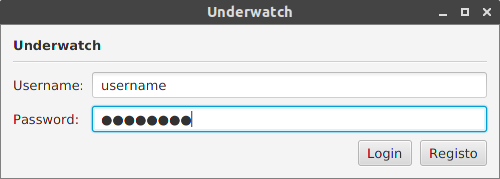
\includegraphics[width=180px]{Interface/menu_autenticacao.png}
\caption{Menu Inicial}
\label{menu_inicial}
\end{figure}

\subsubsection{Menu de Estatísticas}

Este menu possibilita ao utilizador visualizar os seus dados estatísticos: valor de \textit{rank} e número de jogos efetuados e ganhos.
Ao carregar no botão \texttt{Jogar} é enviada ao servidor uma mensagem que indica a vontade de jogar do utilizador e enquanto não recebe uma mensagem a informá-lo que foi encontrada uma partida é mostrado o menu de espera.
Caso pressione \texttt{Logout}, o utilizador é desconetado.

\begin{figure}[H]
\centering
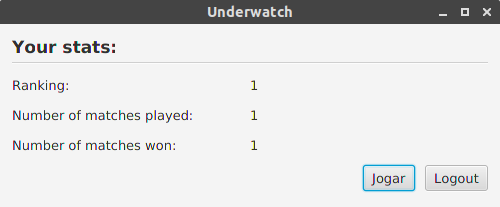
\includegraphics[width=180px]{Interface/your_stats.png}
\caption{Menu de Estatísticas}
\label{menu_estatisticas}
\end{figure}

\subsubsection{Menu de Espera}

\begin{figure}[H]
\centering
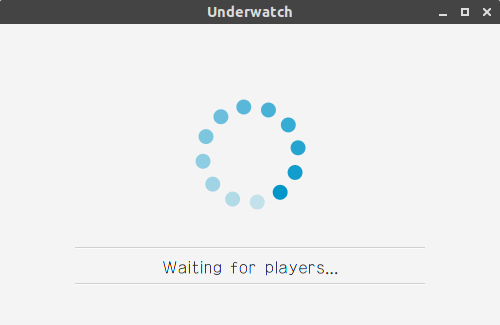
\includegraphics[width=180px]{Interface/loading.png}
\caption{Menu de Espera}
\label{menu_loading}
\end{figure}

\subsubsection{Menu de Escolha de Personagens}

Quando o cliente recebe a mensagem que o informa que foi encontrada uma partida na qual pode participar, surge este menu.
O utilizador pode selecionar, carregando nas imagens, o herói que irá utilizar na partida e são atualizados, em tempo real, os heróis que os jogadores da sua equipa escolheram.
Quando um herói é escolhido fica indisponível e a opacidade da sua imagem é reduzida. 
Note-se ainda que os jogadores podem alterar em qualquer altura o seu herói escolhido, sendo possível optar por qualquer outro ainda disponível, até que o tempo de escolha (que pode ser visto abaixo) se esgote.
Se todos os jogadores tiverem escolhido um herói, aparece o menu de equipas. Em caso contrário, o jogo é cancelado e voltamos ao menu de estatísticas.

\begin{figure}[H]
\centering
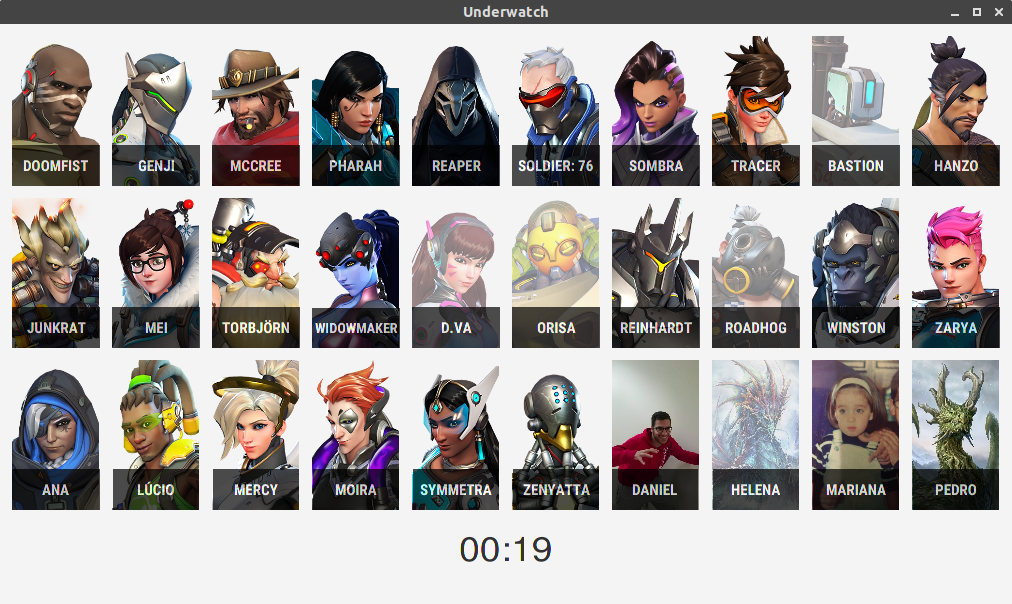
\includegraphics[width=400px]{Interface/menu_escolha_personagens.png}
\caption{Menu de Escolha de Personagens}
\label{menu_personagens}
\end{figure}

\subsubsection{Menu de Equipas}

Este menu permite ao utilizador saber quem são os seus colegas de equipa e os seus adversários, assim como as personagens escolhidas por cada um. 
Passado algum tempo é substituído pelo menu de jogo.

\begin{figure}[H]
\centering
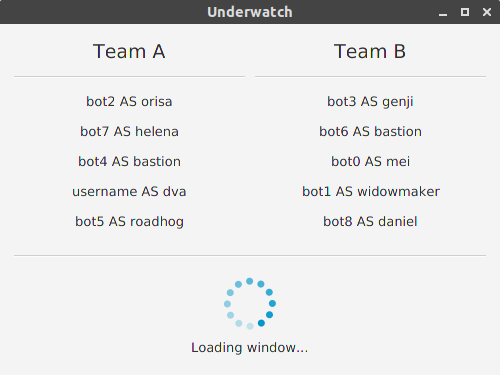
\includegraphics[width=180px]{Interface/display_teams.png}
\caption{Menu de Equipas}
\label{menu_equipas}
\end{figure}

\subsubsection{Menu de Jogo}

O menu de jogo tem a função de simular o tempo de jogo. Quando este termina, regressamos ao menu de estatísticas,  que terá a informação atualizada, resultante do jogo que terá acabado de decorrer.

\begin{figure}[H]
\centering
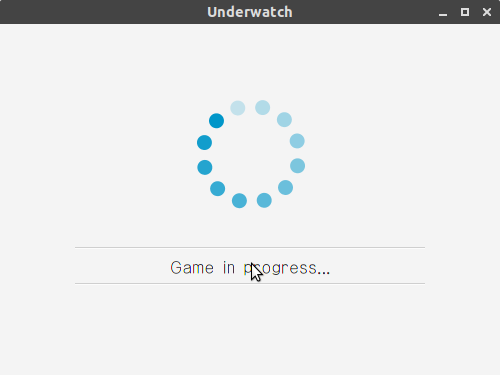
\includegraphics[width=180px]{Interface/game_in_progress.png}
\caption{Menu Inicial}
\label{menu_jogo}
\end{figure}


\section{Conclusão}
Neste trabalho pudemos utilizar e ver em prática os vários conceitos de controlo de concorrência, assim como a implementação de um sistema que se serve da arquitetura Cliente-Servidor, elementos estes 
que compõe a aplicação distribuída aqui desenvolvida. O servidor suporta a ligação entre si e vários clientes, sendo criadas \textit{threads} de execução para lidar com os processos de escrita e leitura 
entre ambas as partes envolvidas. O processo de comunicação (operações de escrita e leitura), suportado pelas \textit{threads}, utiliza \textit{sockets} TCP. Para além da comunicação, também o próprio jogo 
e as partidas que nele decorrem são suportadas por \textit{threads}, na qual participam jogadores humanos, através da interface gráfica desenvolvida, ou \textit{bots}, criados para facilitar a verificação das 
funcionalidades do \textit{software} criado, evitando a necessidade de ter um ou vários jogadores humanos a interagir com múltiplas interfaces. Assim, apesar de haver sempre espaço para melhorias, julgamos ter atingido todos os objetivos propostos.

\end{document}